\begin{thm}{013}{\hosi 4}{灘中入試 (2012)}
 合同な二つの三角形を図のように置きます。このときABの長さは何cmですか。
 \begin{center}
  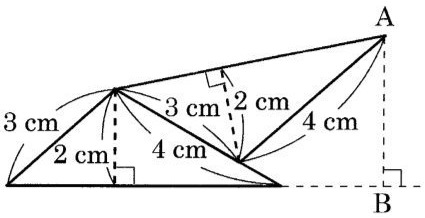
\includegraphics[width=0.6\linewidth]{../problems/Q_013/Q_013.jpg}
 \end{center}
\end{thm}

下図のように点C, D, P, Q, Rをとる。辺ACの延長と辺QDの交点を点E、点Cから辺QDに下した垂線の足を点Fとする。
\begin{figure}[H]
 \centering
 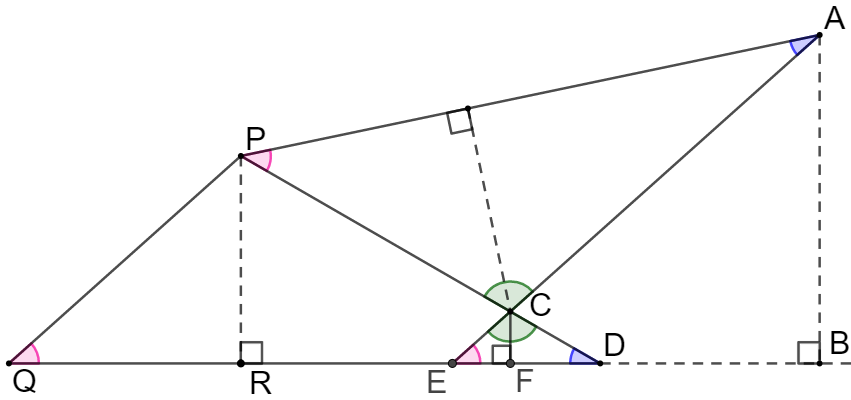
\includegraphics[width=0.6\linewidth]{../problems/Q_013/A_013.png}
\end{figure}
このとき、$\angle\mr{PAC}=\angle\mr{EDC}$と$\angle\mr{PCA}=\angle\mr{ECD}$によって、$\triangle\mr{PCA}\sim\triangle\mr{ECD}$が成り立つ。これによって$\mr{CD}:\mr{CE}=4:3$であり、$\mr{CD}=\mr{PD}-\mr{PC}=1$であるから、$\mr{CE}=\dfrac{3}{4}$。さらに、$\angle\mr{CED}=\angle\mr{CPA}=\angle\mr{PQR}$であることから、
\[ \triangle\mr{PQR}\sim\triangle\mr{CEF}\sim\triangle\mr{AEB} \]
が成り立つ。よって$\mr{AE}:\mr{AB}=3:2$で、$\mr{AE}=\mr{AC}+\mr{CE}=\dfrac{19}{4}$だから、$\mr{AB}=\dfrac{19}{6}$